\documentclass[10pt,a4paper]{report}
\usepackage[utf8]{inputenc}
\usepackage[left=2cm,right=2cm,top=2cm,bottom=2cm]{geometry}
\usepackage{amsmath}
\usepackage{amsfonts}
\usepackage{amssymb}
\usepackage{color}
\usepackage{array}
\usepackage{graphicx}
\usepackage{caption} 
\usepackage{graphicx}
\usepackage[french]{babel}
\usepackage{hyperref}
\usepackage{algorithm}
\usepackage{algorithmic}

\begin{document}
\title{\textbf{ {\Huge Surveillance du Golfe de Gascogne}}}

\maketitle

\pagebreak

\begin{LARGE}
\textbf{Introduction}
\end{LARGE}



\bigskip

Le but de ce projet est de détecter des intrus dans une zones maritime donnée. Ici, nous allons nous intéressé au Golfe de Gascogne. Nous allons donc utiliser un groupe de robots équipés de GPS et nous allons implémenter des algorithmes et un stratégie pour assurer la sureté d'une zone. 

\bigskip

Nous allons avoir plusieurs hypothèses de départ:
\begin{itemize}
\item Nous supposeront que l'étude peut être simulée dans un monde en deux dimensions.
\item Les intrus auront une vitesse constante tout au long de la simulation.
\item Tous les robots pourront voir autour d'eux sur une distance $d_{i}$ et détecter si  un intrus est présent sur cette zone.
\item Nous définissons une zone sûre comme un ensemble de points où un intrus ne peut se trouver.
\end{itemize}

\bigskip

Nous allons donc présenter au final deux livrables:
\begin{itemize}
\item Une simulation théorique faite en grande partie en langage python qui permettra de déterminer la pertinence de nos algorithmes.
\item Un simulation sur des robots chars disponibles au club robotique de l'ENSTA Bretagne.
\end{itemize}

\chapter{Quelles stratégies ont été retenues}

Expliquer comment nous allons répondre aux exigences

1) Description de la trajectoire retenue
2) Méthode retenues (OpenCV / théorie des intervalles )


\chapter{Mise en œuvre des solutions}

\paragraph{Trajectoire elliptique}

\paragraph{Répartition des bateaux}
Dans un premier temps, nous avions penser à répartir les bateaux avec un espacement régulier selon l'abscisse curviligne de l'ellipse.
Cette méthode étant finalement très difficile à mettre en place d'un point de vue mathématique et algorithmique, cette solution a été abandonnée. Il aurait fallu, pour se faire, approximer les intégrales de Wallis par un développement limité assez complexe, ce qui implique un temps de programmation important et un temps de calcul beaucoup trop long pour une simple étude de faisabilité.
C'est pour cela que nous avons décidé de nous orienter vers un retard angulaire sur chacun des robots. Ainsi, chaque robot suit le robot précédent avec un retard angulaire fixe dépendant du nombre de robots parcourant l'ellipse. Cela implique que les robots vont être d'autant plus proches les uns des uns qu'il sont près des apogées de l'ellipse, et d'autant plus éloignés aux périgées.
Néanmoins, malgré la non-linéarité du placement des robots, nous n'avons pas de rupture de la zone de détection. En effet, comme les robots vont plus vite aux périgées, la trace qu'ils "laissent" est plus grande, et inversement aux apogées. De ce fait, on peut garantir la sécurité de la zone à surveiller, même si les robots ne sont pas régulièrement espacés.


\section{Évolution de la consigne au cours du temps}

Alice / Eric / Chuch

\section{Regulation of multiples real robots for demonstration of concept}


\section{Regulation of the robot pack}

Two methods have been studied and implemented to regulate the pack of robots. The first is a method by artificial potential field, robust and easy to debug. This method was chosen to regulate the real robots on the play field. The second method is a method of looping linearisation, very efficient. This method was chosen for the simulation because its integration in a simulation is easier than on robots.

\subsection{Artificial potential field}
Let $p_{robot}$ be the position of our considered robot, let $p_{target}$ and $v_{target}$ be the position and speed of the target we want the robot to reach.
We can consider the robot and the target as two particles of opposite charge, and then compute the potential field between them. In case of obstacles, we can consider them as particles of same charge than the robot's.
The potential field method calculate the instantaneous speed vector $w(p_{robot},t)$ the robot need to reach (or at least follow) the target. To compute that speed, we use the potential $V$ between the robot and the target :\\
\[ V(p_{robot}) = v^T_{target}. p_{robot} + \|p_{robot}-p_{target}\|^2 \]
And compute the gradient of that potential to find the order $w(p_{robot},t)$:
\[w(p_{robot},t) = -grad(V(p_{robot})) = -\frac{dV}{dP}(p)^T\]
So :
\[w(p_{robot},t) = v_{target}-2.(p_{robot}-p_{target})\]
For w, we compute the objective speed and course:
\[\bar{v} = |w\| \]
\[\bar{\theta} = tan(\frac{w_y}{w_x})\]

Alice / Eric / Chuch ou Totoboule / Sylvain selon la solution retenue

\section{Description du fonctionnement du simulateur}

Totoboule / Sylvain + Image à faire

\section{Secure zone estimation with interval analysis}

\subsection{Basics and Usefulness of Interval Arithmetics}
 
Normal solver equation are efficient with linear sytems but in a real environment 

\subsection{Thick Functions}

\subsection{Special Test for Gascogne Surveillance}

\begin{algorithm}
\caption{Is $\mathbf{X} \subseteq \mathbb{S}$ , $\mathbb{S} =$ Secure Zone and $\mathbf{X} \in \mathbb{R^{\textnormal{\ensuremath{2}}}}$ }
\begin{algorithmic}
\REQUIRE $range \geq 0 \vee \mathbf{X} \neq \emptyset$
\STATE $Xmx \leftarrow max([0,0], sign( (X[0]-m[0].ub())*(X[0]-m[0].lb()))) * \
              min((X[0]-m[0].lb())^{\textnormal{\ensuremath{2}}},(X[0]-m[0].ub())^{\textnormal{\ensuremath{2}}} )$
\STATE $ Xmy \leftarrow max([0,0], sign( (X[1]-m[1].ub())*(X[1]-m[1].lb()))) * min((X[1]-m[1].lb())^{\textnormal{\ensuremath{2}}},(X[1]-m[1].ub())^{\textnormal{\ensuremath{2}}} )$
\STATE $Xm \leftarrow Xmx + Xmy $
\STATE $Xp \leftarrow max((X[0]-m[0].lb())^{\textnormal{\ensuremath{2}}},(X[0]-m[0].ub())^{\textnormal{\ensuremath{2}}}) + \
                  max((X[1]-m[1].lb())^{\textnormal{\ensuremath{2}}},(X[1]-m[1].ub())^{\textnormal{\ensuremath{2}}})$
\STATE $Xub \leftarrow Xp | Xm$
\IF{$Xub \cap \mathbb{[ \,\textnormal{0},\textnormal{range}^{\textnormal{\ensuremath{2}}}] \,} =  \emptyset $}
\RETURN $\textnormal{OUT}$
\ELSIF {$Xub \subseteq \mathbb{[ \,\textnormal{0},\textnormal{range}^{\textnormal{\ensuremath{2}}}] \,} $}
\RETURN $\textnormal{IN}$
\ELSE
\IF{ $\textnormal{range}^{\textnormal{\ensuremath{2}}} - Xp.ub() < \textnormal{0}] $}
\IF{ $Xm - \textnormal{range}^{\textnormal{\ensuremath{2}}} \subseteq \mathbb{[ \,-\infty,\textnormal{0}] \,}$}
\RETURN $\textnormal{MAYBE}$
\ELSE
\RETURN $\textnormal{UNKNOWN2}$
\ENDIF
\ELSE
\RETURN $\textnormal{UNKNOWN}$
\ENDIF
\ENDIF
\end{algorithmic}
\end{algorithm}

Differente result In testing : \newline

\begin{center}
\begin{tabular}{|m{0.10\linewidth}|m{0.5\linewidth}|}
\hline
 Symbol & Meaning  \\ \hline
 0 & Box is not in the Secure Zone  \\ \hline
 1 &  Box is in the secure zone \\ \hline
 ? &  Box may be in the secure zone  \\ \hline
[0,?] & Box may be in the secure zone \\ \hline
[?,1] & Box may be in the secure zone\\ \hline
[0,1] & Box may be in the secure zone or out \\ \hline
    
   
\end{tabular}
\end{center}


\begin{center}
\begin{tabular}{|m{0.10\linewidth}|m{0.07\linewidth}|m{0.07\linewidth}|m{0.07\linewidth}|m{0.07\linewidth}|m{0.07\linewidth}|m{0.07\linewidth}|}
\hline
Test1/Test2 & 0 & 1 & ? & [0,?] &  [?,1] & [0,1] \\ \hline
          0 & 0 & 1 & ? & [0,?] &  [?,1] & [0,1]  \\ \hline
          1 &   & 1 & 1 &   1   &    1   &   1  \\ \hline
          ? &   &   & ? &   ?   &  [?,1] & [?,1] \\ \hline
      [0,?] &   &   &   & [0,?] &  [?,1] & [0,1] \\ \hline
      [?,1] &   &   &   &       &  [?,1] & [?,1] \\ \hline
      [0,1] &   &   &   &       &        & [0,1]  \\ \hline
    
   
\end{tabular}
\end{center}


\section{Prise en compte du passé grâce à OpenCV}

Maël / Khadim / David  ... A vous de choisir vos sous-sections

\subsubsection{Pavage des images}

\subsubsection{Érosion des zones de sureté}


\chapter{Réalisation de test sur robot char}
Benoit / Maxime / Pierre ... A vous de choisir vos sections

Pour la réalisation d'une simulation sur des robots, nous avons du implémenter un architecture afin de permettre à nos programme de gérer d'une part nos robots et d'autre part de voir si le résultat théorique correspond aux résultats expérimentaux.

\medskip

Nous aboutissons au final à l'architecture suivante:

\bigskip

\begin{figure}[ht]
\centering
    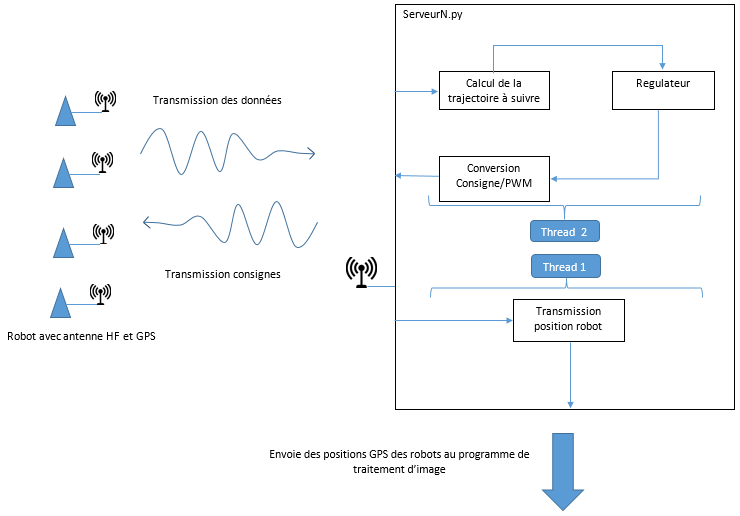
\includegraphics[scale=0.8,angle=0]{SyntheseExp.png}
    \caption{Architecture mise en place pour la simulation sur robot char.}
    \label{fig:SyntheseExp}
\end{figure}

\bigskip

\section{Matériel}
\subsection{GPS}
ici la description des GPS utilisés
\subsection{Robot}
ici la description des robots et des récepteurs
\section{Analyse des trames GPS}
\textcolor{blue}{\textit{Pierre JACQUOT}}

In order to get the GPS coordinates of each robots we decided to use the \textit{GPRMC} sentence send by the GPS's emitter. The exemple below show the structure of a \textit{GPRMC} sentence : \
\begin{center}
\begin{tabular}{|m{0.05\linewidth}|m{0.06\linewidth}|m{0.07\linewidth}|m{0.07\linewidth}|m{0.08\linewidth}|m{0.07\linewidth}|m{0.07\linewidth}|m{0.04\linewidth}|m{0.08\linewidth}|m{0.1\linewidth}|m{0.07\linewidth}|}
\hline
    081836 & A & 3751.65 & S & 14507.36 & E & 000.0 & 360.0 & 130998,01 & 011.3 & E*62  \\ \hline
     UTC & Data status & Latitude & N or S & Longitude & E or W & Speed (knots) & Track made good &  UT Date & Magnetic Variation & E or W and Checksum \\ \hline

\end{tabular}
\end{center}
The most valuable data are the latitude, the longitude, the speed over ground (in knots) ant the time stamp. In order to get those different data, we used the python package pynmea, which allows to easily get and parse a GPS sentence. \\
However, the longitude and latitude obtained using this specific sentence have a particular structure that we had to changed to make them easier to manipulate and compute in our algorithm. The example below show how the longitude and latitude are originally formatted :
\
\begin{itemize}
  \item Longitude  : \textit{12311.12,W} which means Longitude 123 degree. 11.12 min West
  \item Latitude : \textit{4916.45,N} which means Latitude 49 degree 16.45 min North
\end{itemize}

In order to ease the computation, our program automatically convert the longitude and latitude in degrees, take into account the cardinal direction associated with each coordinates.
These cardinal directions North and South for the latitude and East and West for the longitude, let us know respectively on which side of the Greenwich (or prime) meridian we are located and on which side of the equator we are located. As a matter of fact, we will have in Brest a "negative" latitude and a positive longitude, due to our positioning regarding the equator and Greenwich meridian.\\

Our program not only give the coordinates in degrees but also convert them into UTM (Universal Transverse Mercator) coordinates. This new set of coordinates allow a localisation of the robot in a flat local coordinates system and maybe more easy to use as they are just decimal numbers. The UTM system itself, consist in a subdivision of the world in different sectors which can be consider as flat, and with a specific system of coordinates.
The figure below show the subdivision of France: \

\begin{center}
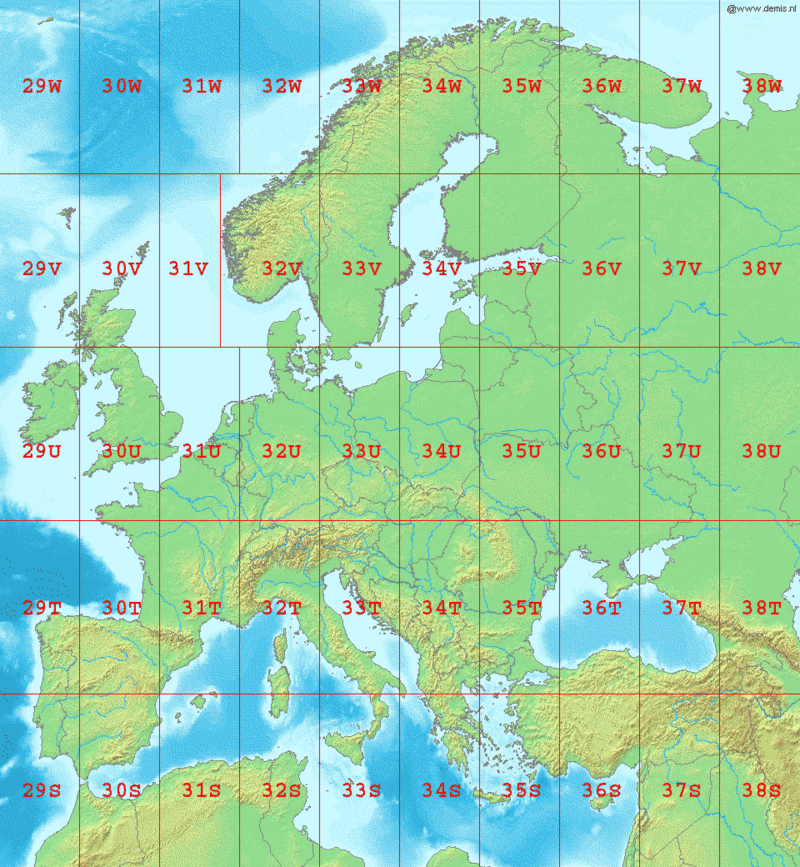
\includegraphics[scale=0.2]{secteurUTM.png} 
\captionof{figure}{Secteur UTM}
\label{fig1}
\end{center}

This figure show that we are currently in the sector 30. Whereas,in order to compute UTM coordinates, we need first to choose a geodesic system representing the Earth. For this project we chose the WGS-84 system which is most commonly used.


\section{Structure du code}

Quatre scripts python: GPS2.py, commande.py, testserial.py et ServeurN.py

\section{Résultats}



\end{document}
